% vim: set textwidth=78 autoindent:
% !TeX root = user_guide.tex

\section{Schnelles Drucken Plugin}
\label{quickprint}
\index{Plugins!Schnelles drucken}

% when the revision of a chapter has been finalized, 
% comment out the following line:
% \updatedisclaimer

Das Plugin \toolbtntwo{quick_print}{Schnelles Drucken} Plugin erlaubt es, das
aktuelle Kartenfenster mit minimalem Aufwand in ein PDF zu exportieren. Der
Benutzer gibt dazu nur einen Kartentitel, einen Kartennamen und die
Seitengr��e an (siehe Abbildung~\ref{fig:quickprint}). F�r mehr Kontrolle
�ber das Kartenlayout steht das Print Composer Plugin (siehe
Kapitel~\ref{label_printcomposer}) zur Verf�gung.

\begin{figure}[ht]
   \begin{center}
   \caption{Schnelles Drucken Dialog \nixcaption}
   \label{fig:quickprint}\smallskip
   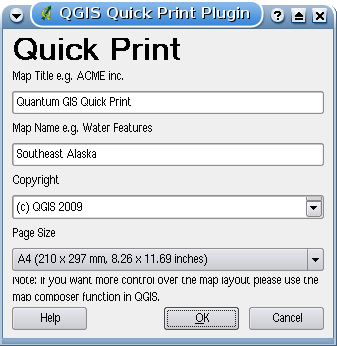
\includegraphics[clip=true, width=6cm]{quick_print_dialog}
\end{center}
\end{figure}

\begin{figure}[ht]
   \begin{center}
   \caption{DIN A4 Schnelldruck als PDF mit den QGIS Beispieldaten \nixcaption}
   \label{fig:quickprint_result}\smallskip
   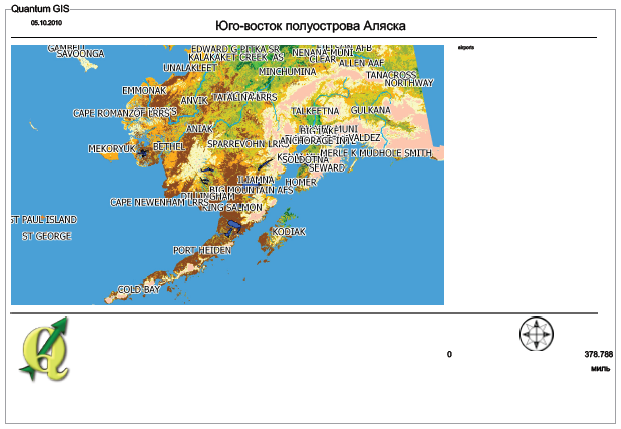
\includegraphics[clip=true, width=9cm]{quick_print_result}
\end{center}
\end{figure}

\FloatBarrier
